\documentclass[a4paper,11pt]{jsarticle}


% 数式
\usepackage{amsmath,amsfonts,amssymb}
\usepackage{bm}
% 画像
\usepackage[dvipdfmx]{graphicx}
\usepackage{siunitx}
\usepackage{wrapfig}
\usepackage{cases}
\makeatletter
\newcommand{\figcaption}[1]{\def\@captype{figure}\caption{#1}}
\newcommand{\tblcaption}[1]{\def\@captype{table}\caption{#1}}
\makeatother

\begin{document}

\title{}
\author{}
\date{\today}
\maketitle

\begin{figure}[b]
  \centering
  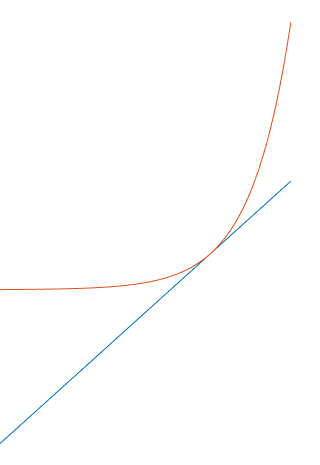
\includegraphics[width = 0.4\textwidth]{210425_spinNumの評価_01.png}
  \caption{}
  \label{}
\end{figure}

$y=f(x)=\exp(px + q) + r$と$y = ax$が$x=b$で接するには
\begin{align*}
  \begin{cases}
    f(b) = ab \\
    f'(b) = a
  \end{cases}
\end{align*}
を満たす必要があるから
\begin{align*}
  &\begin{cases}
    \exp(pb + q) + r = ab\\
    p\exp(pb + q)=a
  \end{cases}
  \\
  &\therefore\begin{cases}
    \frac{a}{p} + r = ab\\
    pb + q = \log(\frac{a}{p})
  \end{cases}
  \\
  &\therefore\begin{cases}
    r = ab - \frac{a}{q}\\
    q = \log\frac{a}{p} - pb
  \end{cases}
\end{align*}


\end{document}